\section{Нейросетевая регрессия (случай одного класса)}

Как отмечалось в разделе~\cref{subsec:ch1/neural_approximation}, многослойный персептрон с кусочно-линейной функцией активации (в частности, с активацией вида \(|x|\)), при наличии \(L\) скрытых слоёв, каждый из которых содержит \(k\) нейронов, способен осуществлять \(\epsilon\)-приближенную аппроксимацию любой непрерывной функции на компакте. При этом конструкция такой нейросети задаёт иерархическое (по слоям) разбиение компакта \([0, 1]^d\) на \(O(k^{dL})\) ячеек, внутри которых выход нейросети представляет собой линейную функцию. Вычисление значения такой нейросети в произвольной точке \(x \in [0, 1]^d\) требует только последовательного выполнения операций скалярного умножения и сравнения, что обеспечивает высокую вычислительную эффективность полученной модели.

Для дальнейшего анализа введём обобщённую задачу регрессии, сформулированную следующим образом. Пусть имеется исходный набор наблюдений \(\{X_i\}_{i=1}^n\), представляющий собой независимые одинаково распределённые случайные величины на компакте \([0, 1]^d\) с неизвестной ограниченной плотностью распределения \(f(X)\). Этот набор можно интерпретировать как наблюдения некоторого целевого процесса, подлежащего моделированию. Для каждого такого наблюдения \(X_i\) положим значение метки \(Y_i = 1\).

Дополнительно сформируем ``фоновые`` наблюдения \(\{X_i\}_{i=n+1}^{2n}\), представляющие собой независимые одинаково распределённые случайные величины с равномерной плотностью распределения \(p(X)\) на том же компакте \([0,1]^d\). Для этих наблюдений положим значения \(Y_i = 0\). В результате будет получен комбинированный набор данных \(\{(X_i, Y_i)\}_{i=1}^{2n}\) мощности \(2n\).

Рассмотрим теперь задачу построения аппроксимирующей полносвязной нейросети \(c_n(X)\), решающей задачу регрессии в классе моделей фиксированной сложности, аналогичную задаче \cref{eq:perceptron_optimization}. Требуется найти такую нейросеть \(c_n^*(X)\), минимизирующую среднеквадратичную ошибку на объединённом наборе данных:

\begin{equation}
    \label{eq:unary_perceptron_optimization}
    \sum_{i=1}^{2n} \left(c_n(X_i) - Y_i\right)^2 \rightarrow \min_{c_n},
\end{equation}

\noindent где минимум берётся по всем полносвязным нейросетям, общее число нейронов в которых не превышает заданного порогового значения \(kL + 1\).

Пусть в результате построения \(c_n^*(X)\) на компакте \([0, 1]^d\) получено разбиение на \(N\) ячеек \(K = \{K_1, K_2, \dots, K_N\}\). Введём далее кусочно-постоянную функцию \(h_n(X)\), принимающую постоянные значения внутри каждой ячейки \(K_r\), и сформулируем задачу приближённой оценки вероятности принадлежности наблюдения классу \(Y = 1\) в виде:

\begin{equation}
    \label{eq:unary_histogram_optimization}
    \sum_{i=1}^{2n} \left(h_n(X_i) - Y_i\right)^2 \rightarrow \min_{h_n}
\end{equation}

Как и в \cref{eq:histogram_optimization}, задача~\cref{eq:unary_histogram_optimization} может быть решена независимо в каждой ячейке \(K_r\), при этом оптимальное значение \(h_n^*(X)\) в данной ячейке определяется соотношением:

\begin{equation}
    h_n^*(X) = \frac{n_1(X)}{n_1(X) + n_0(X)},
\end{equation}

\noindent где \(n_1(X)\) -- количество наблюдений с меткой \(Y = 1\) в ячейке, содержащей точку \(X\), а \(n_0(X)\) -- количество фоновых наблюдений (с меткой \(Y = 0\)) в той же ячейке.

Пример вычисления функции гистограммной регрессии показан на рисунке~\cref{fig:unary_histogram_evaluation}.

\begin{figure}[ht]
    \centerfloat{
        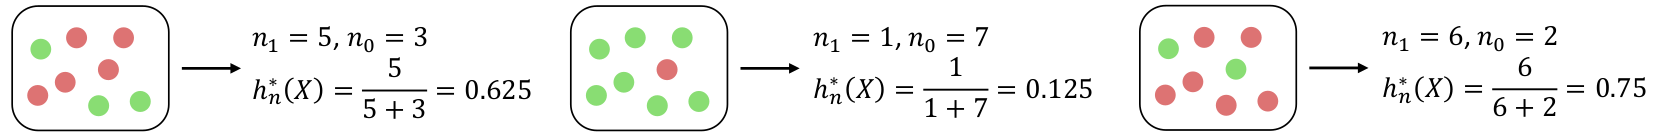
\includegraphics[width=\linewidth]{Dissertation/images/ch1/bayesian_classifier_approximation/histogram_evaluation.png}
    }
    \caption{Пример вычисления \(h_n^*(X)\) в некоторой ячейке \(K_r\) в унарном случае}
    \label{fig:unary_histogram_evaluation}
\end{figure}

Полученная функция \(h_n^*(X)\) представляет собой оценку апостериорной вероятности принадлежности к целевому распределению \(f(X)\), основанную на локальной структуре данных в разбиении, индуцированном нейросетевой аппроксимацией.